\documentclass[a4paper]{article}

\usepackage[brazil]{babel}
\usepackage[utf8]{inputenc}
\usepackage{amsmath,amsfonts,amssymb,latexsym,mathrsfs,amsthm,amstext,bezier,amscd}
\usepackage{graphicx}
\usepackage{indentfirst}
\usepackage{setspace}

\begin{document}
\thispagestyle{empty}

\begin{titlepage}
	\vfill
	\begin{center}
		\parbox{6cm}{
\includegraphics[scale=0.2]{logo.png}}\\
		\begingroup
		\fontsize{12pt}{0pt}\selectfont
		{\large \textbf{INSTITUTO FEDERAL DE EDUCAÇÃO, CIÊNCIA E TECNOLOGIA DO CEARÁ}}\\[0.2cm]
		\fontsize{12pt}{0pt}\selectfont
		{\large \textbf{IFCE CAMPUS MARACANAÚ}}\\[0.2cm]
		\fontsize{12pt}{0pt}\selectfont	
		{\large \textbf{BACHARELADO EM CIÊNCIA DA COMPUTAÇÃO}}\\[4cm]
		\fontsize{12pt}{0pt}\selectfont
		{\large \textbf{THIAGO MAGALHÃES FURTADO}}\\[3.5cm]
		\fontsize{12pt}{0pt}\selectfont
		{\large \textbf{Avaliação de Acessibilidade em Portais de Notícias}}\\[3.5cm]
		\fontsize{12pt}{0pt}\selectfont
		{\large \textbf{MARACANAÚ}}\\[0.2cm]
		\fontsize{12pt}{0pt}\selectfont
		{\large \textbf{2021}}
		\endgroup
	\end{center}
\end{titlepage}

\begin{titlepage}
	\vfill
	\begin{center}
		\fontsize{12pt}{0pt}\selectfont
		{\large \textbf{THIAGO MAGALHÃES FURTADO}} \\[2.5cm]
		\fontsize{12pt}{0pt}\selectfont
		{\large \textbf{Avaliação de Acessibilidade em Portais de Notícias}}\\[3cm]
		
		\hspace{.45\textwidth} %posiciona a minipage
		\begin{minipage}{.5\textwidth}
			\large Trabalho de Conclusão de Curso apresentado ao curso de Bacharelado em Ciência da Computação do Instituto Federal de Educação, Ciência e Tecnologia do Ceará (IFCE) - Campus Maracanaú, como requisito parcial para obtenção do Título de Bacharel em Ciência da Computação.\\[1cm]
			Prof. Dr. Otávio Alcântara de Lima Junior.
		\end{minipage}
		\vfill
		\vspace{2cm}		
		\large \textbf{Maracanaú - CE}
		
		\large \textbf{2021}
	\end{center}
\end{titlepage}

\begin{titlepage}
	\begin{center}
		\tableofcontents
	\end{center}
\end{titlepage}
\begin{titlepage}
\section{INTRODUÇÃO}
\fontsize{12pt}{0pt}\selectfont
\onehalfspacing
Estamos vivendo em uma época em que a tecnologia tem avançado bastante, isso é notório se nós analisarmos as três últimas décadas, durante as quais o mundo entrou na chamada era da informação. Assim, os computadores, a Internet, os acessos aos sites e o número de usuários, em todo o mundo, têm tido avanços significativos. Esses avanços possibilitam, para a nossa sociedade, uma prestação de serviço e uma obtenção de informação rápida. Porém, muitos sites não possibilitam uma navegação agradável e tranquila à todos, já que alguns usuários tem dificuldade para acessá-los, por possuírem alguma deficiência, a OMS relata que 15\% da população mundial tem alguma deficiência [1].

Dentre a diversidade de conteúdo da Internet, pode-se destacar os portais de noticiais como ferramentas importantes para divulgação de informação de qualidade para a sociedade. Porém essas plataformas digitais precisam alcançar todos os usuários, inclusive os PCDs(pessoas com deficiência). Para avaliar a acessibilidade desses sites, é necessário a aplicação de diretrizes de acessibilidade que são propostas por instituições e governos. Por exemplo, a eMAG é uma diretriz proposta pelo governo brasileiro em 2004, utilizada por algumas plataformas digitais nacionais [2].

Outra diretriz usada atualmente é a WCAG (Web Content Accessibility Guidelines), que já está na sua segunda versão, isto é, a WCAG 2.0. A WCAG possuí doze diretrizes organizadas em quatro princípios diferentes, possuindo algumas recomendações para cada princípio [3], que são indispensáveis em qualquer plataforma digital, inclusive nos sites de notícia.

O WCAG é um padrão adotado em diversos trabalhos de avaliação de acessibilidade, em [4], foi avaliado a acessibilidade dos vídeos na plataforma online de curso MOOC. Foram analisados os vídeos através da verificação do uso de uma alternativa à informação visual, de audiodescrição, transcrições, de uma fonte boa, com um tamanho de letra razoável e de alto-contraste. Em o [5] e em [6] foi analisado a existência de acessibilidade dos sites de ensino do nível superior da Índia utilizando o WCAG e uma ferramenta de avaliação, chamada de TAW. Em 2016, foi feito um acompanhamento, por meio do WCAG, dos serviços de governo eletrônico da Arábia Saudita, com o objetivo de analisar o nível de conscientização e as políticas do próprio governo [7]. Por fim, em [8], foi feito uma analise de um método heurístico existente para investigar o nível de acessibilidade de 40 sites em relação aos usuários com baixa visão juntamente com a diretriz WCAG 2.1, o método utilizado foi proposto por Brajnik.

Este artigo propõe a avaliação de acessibilidade de dez dos principais portais de notícias brasileiros, que tem um papel importantíssimo em relação ao repasse de informação para o público em geral, inclusive para os usuários PCDs, supondo que eles não atendem de forma plena os requisitos desse público. Para isso será proposto uma avaliação da acessibilidade de dez sites de notícia para pessoas que possuem algum grau de deficiência visual ou auditiva. A pesquisa tem o intuito de analisar os sites, de forma plena, para quantificar o grau de acessibilidade de cada um. Assim, o objetivo geral do trabalho é avaliar sites de notícias que possuem formas de acessibilidade digital, sejam completamente, parcialmente ou não acessíveis para a deficiência visual e para a deficiência auditiva. A metodologia empregada consiste em caracterizar a definição de acessibilidade digital, verificar as formas de deficiência existentes que afetam a usabilidade dos sites, apresentando a diretriz WCAG, escolhendo os princípios destinados aos deficientes visuais e auditivos para mensurar os sites de notícias em relação a acessibilidade.

O restante do artigo está organizado da seguinte forma. Na seção 2 será mostrado a metodologia que será aplicada para fazer a analise dos sites. Na seção 3 será apresentado o estado da arte de avaliação de acessibilidade em sites usando as diretrizes, mostrando quais diretrizes usaram e em quais plataformas aconteceram as suas pesquisas. Na seção 4 serão explicadas as formas de deficiência existentes que afetam a usabilidade dos sites. Na seção 5 será analisado a diretriz WCAG. Na seção 6 será apresentado os pontos fortes e fracos dos sites de notícias relacionado com a acessibilidade web através da análise da diretriz com o propósito de fazer sugestões de melhorias. Por fim, na seção 7 será apresentada uma discussão sobre os resultados da avaliação de acessibilidade e a conclusão do trabalho.

\section{METODOLOGIA}
Os sites notícia foram escolhidos por serem bastante importantes para a sociedade atual, informando cada pessoa que as acessa. Sendo assim, a metodologia, que será aplicada para que os objetivos sejam alcançados, será:

1 - Mostrar e explicar as formas de deficiência visual e auditiva;

2 - Analisar a WCAG;

3 - Pontuar os princípios e as especificações da diretriz WCAG;

4 - Apontar as principais formas acessibilidade, usando a diretriz WCAG;

5 - Escolher dez sites de notícias do Brasil;

6 - Fazer um levantamento da acessibilidade de cada site de acordo com as especificações;

7 - Fazer um comparativo entre os sites;

8 - Apresentar a conclusão tirada dos dez sites escolhidos, propondo melhorias em cada um deles.

Todos os passos da metodologia que será aplicada estão descritos na Figura 1.\\

Figura 1 - Fluxograma das etapas da metodologia\\[-0.7cm]
\begin{center}
	\parbox{10cm}{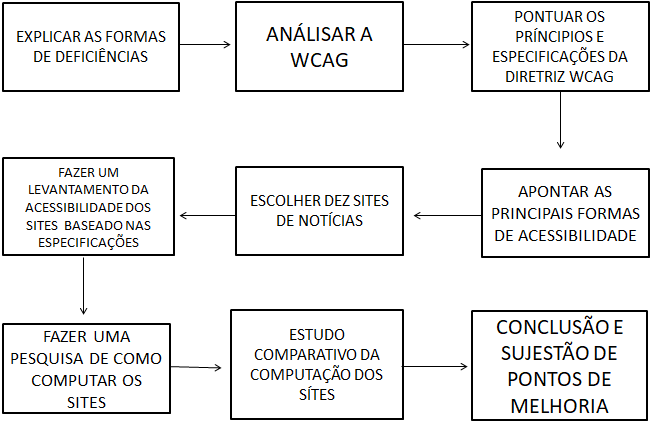
\includegraphics[scale=0.4]{Fluxograma - Metodologia TCC.png}}
\end{center}

Portanto, esse será o caminho percorrido por esse artigo. A seguir, será apresentado os trabalhos relacionados sobre acessibilidade digital.

\section{TRABALHOS RELACIONADOS}
Há uma grande produção nessa área, contudo serão concentrados os artigos publicados em revistas. Será mostrado os artigos que tratam sobre as diretrizes utilizadas nos respectivos estudos e sobre as propostas de avaliação em diversas áreas, sejam elas em portais de notícia ou não.

\subsection{Diretrizes}
Sobre as diretrizes, serão apresentados alguns trabalhos que focaram em duas diretrizes, que são a eMAG e a WCAG. Os autores artigo [2], definiram que a acessibilidade digital, usando a Organização Mundial da Saúde(OMS), dizendo que, de acordo com a “Convenção sobre os direitos das pessoas com deficiência”, pessoas com deficiência são aquelas que têm incapacidades físicas, mentais, intelectuais ou sensoriais a longo prazo que, em interação com diversas barreiras, podem prejudicar sua participação plena e efetiva na sociedade em igualdade de condições com os outros. Segundo eles, no Brasil existe um decreto de número 5.296 de 2004, que disponibilizou o Modelo de Acessibilidade em Governo Eletrônico (eMAG), que foi utilizado para analisado 107 sites de Instituições Federais de Educação(IFEs) do Brasil. Eles pontuaram alguns elementos importantíssimos para a acessibilidade tiradas da eMAG, como exemplo, atalhos de teclados, alto contraste, barra de acessibilidade, existência do mapa de sítio e páginas de descrição com os recursos de acessibilidade. Porém, concluíram que não foram implementados de maneira satisfatória os pontos de acessibilidade nos portais dos IFEs do país, e que as barreiras ao acesso à informação digital são o resultado da falta de atenção durante o processo de desenvolvimento da tecnologia, ao invés de limitações inerentes a essa tecnologia.

Já sobre a diretriz WCAG, no artigo [1], produzido no ano de 2020, é dito que a acessibilidade na web visa tornar os sites mais acessíveis e utilizáveis pelo maior número de pessoas possível, independentemente de seus conhecimentos, habilidades ou características técnicas, e que a diretriz WCAG, criado pela empresa W3C, é essencial para desenvolvedores e organizações que desejam criar sites e ferramentas de alta qualidade, e não excluir as pessoas de usarem seus produtos e serviços. Então o artigo se propôs a falar sobre esses dois temas, que é explicar a diretriz e mostrar a definição da acessibilidade Web.

A WCAG, publicada pela World Wide Web (W3C) no dia primeiro de outubro de 1994, através da organização chamada World Wide Consortium, que é um consórcio com 450 membros, empresas, organizações independentes e ONGs, tem como objetivo formular padrões para os desenvolvedores criarem seus sites. Segundo o artigo [3], a acessibilidade na web refere-se a recursos de design da web que permitem que as pessoas operem os sites, e que a WCAG 2.0, tem como objetivo eliminar erros de acessibilidade através dos web designers e dos desenvolvedores. Assim, ela serve de apoio para os desenvolvedores a boa prática da acessibilidade web, garantindo um acesso à internet satisfatório, atingindo o maior número de pessoas possível, independente da existência de uma comorbidade física. Por meio desse artigo, vemos que a criação da diretriz WCAG tem uma grande importância, pois, caso os programadores decidam segui-lá, tornarão os sites cada vez mais acessíveis para todo e qualquer ser humano que deseja usá-lo, independente se o usuário possui ou não algum tipo de deficiência, seja ela física, motora ou mental. 

Ainda sobre a diretriz WCAG, existe uma documentação [10], no qual a ultima versão foi publicada em 11 de dezembro de 2008, onde é passada as recomendações, explicando, sucintamente, os seus quatro princípios. Será feito, agora, um esclarecimento dos seus princípios, e, mais na frente, será falado como cumprir as diretrizes e como quantificar os sites. O primeiro princípio é o perceptível, no qual informação e os componentes da interface de utilizador têm que ser apresentados de forma a que os utilizadores as possam entender. Nesse princípio existem quatro diretrizes com suas especificações. As diretrizes determinam que os sites precisam ter alternativas em texto, ter uma mídia dinâmica e contínua, ser adaptável e ser distinguível.

O site ter alternativas em texto significa que ele deve fornecer alternativas em texto para todo o conteúdo não textual de modo que possa ser apresentado de outras formas, de acordo com as necessidades dos utilizadores. Alguns exemplos são caracteres ampliados, braille, fala, símbolos ou uma linguagem mais simples. Ja o site ter um mídia dinâmica ou contínua remete que ele deve fornecer alternativas para conteúdo em multimédia dinâmica ou temporal. A diretriz adaptável diz que deve ser criado um conteúdo que possa ser apresentado de diferentes formas, por exemplo, um esquema de página mais simples, sem perder informação ou estrutura. Por fim, a diretriz distinguível expressa que deve haver uma facilitação dos utilizadores à audição e à visão dos conteúdos nomeadamente através da separação do primeiro plano do plano de fundo. Todas as diretrizes do princípio perceptível estão especificadas e descritas, logo abaixo, na figura 2.\\

Figura 2 - Diretrizes do princípio perceptível\\[-0.7cm]
\begin{center}
	\parbox{11cm}{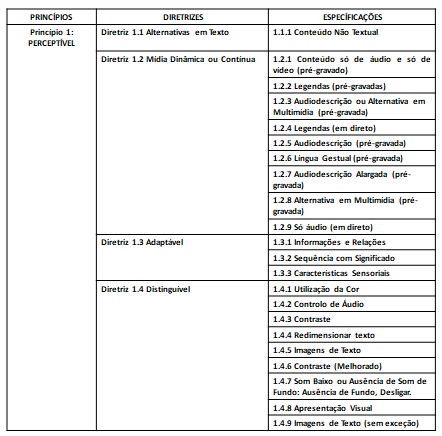
\includegraphics[scale=0.9]{Perceptível.png}}
\end{center}

Já o segundo princípio é o operável, onde é definido os métodos, que possibilitam, para os usuários, uma interação e uma boa navegação pelo conteúdo de forma confortável. O princípio diz que os sites devem usar interfaces apropriadas para os deficientes, isto é, os componentes da interface de utilizador e a navegação têm de ser operáveis. Nesse princípio existem quatro diretrizes com suas especificações. As diretrizes determinam que o site deve ser acessível por teclado, deve ter um tempo suficiente, não deve causar convulsões e ele deve ser navegável.

Dizer que a plataforma digital deve ser acessível por teclado exprime que ela deve ter uma funcionalidade que fique disponível a partir do teclado. Já o site ter um tempo suficiente revela que ele deve proporcionar aos utilizadores um tempo suficiente para lerem e utilizarem o conteúdo. Sobre o site não causar convulsões, pressupõe-se que ele não deve criar conteúdos de uma forma que se sabe que pode causar convulsões em alguns usuários. E, por último, dizer que a página da Internet deve ser navegável, representa que ela deve fornecer formas de ajudar os utilizadores a navegar, localizar conteúdos e determinar o local onde estão. Todas as diretrizes do princípio operável estão especificadas e descritas, logo abaixo, na figura 3.\\

Figura 3 - Diretrizes do princípio operável\\[-0.7cm]
\begin{center}
	\parbox{11cm}{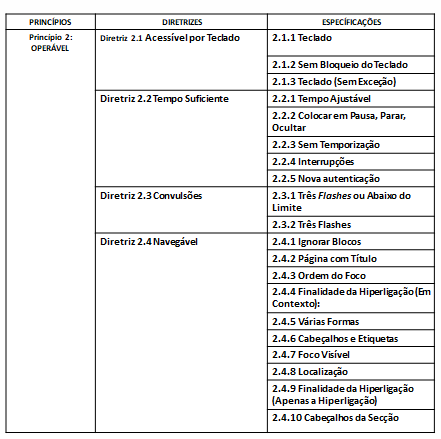
\includegraphics[scale=0.9]{Operável.png}}
\end{center}

O terceiro princípio é o compreensível, que diz que os usuários devem ser capazes de compreender as informações e o funcionamento da interface, com o objetivo do usuário interpretar corretamente o conteúdo da plataforma digital, isto é, a informação e a utilização da interface de utilizador têm de ser compreensíveis. Nesse princípio existem três diretrizes com suas especificações. As diretrizes determinam que o site deve ser legível, deve ser previsível e deve existir assistência na Inserção de Dados.

Dizer que o sítio da Internet deve ser legível simboliza que ele é capaz de tornar o conteúdo textual legível e compreensível. Já falar que o sítio eletrônico tem que ser previsível reflete a ideia de fazer com que as páginas Web apareçam e funcionem de forma previsível. E existir na página Web uma assistência na inserção de dados, retrata que ela deve ajudar os utilizadores a evitar e a corrigir os erros. Todas as diretrizes do princípio compreensível estão especificadas e descritas, logo abaixo, na figura 4.\\

Figura 4 - Diretrizes do princípio compreensível\\[-0.7cm]
\begin{center}
	\parbox{11cm}{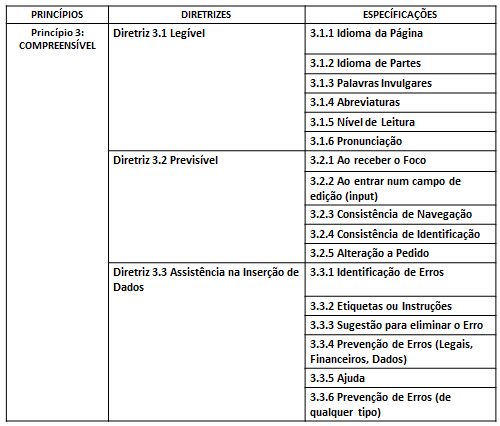
\includegraphics[scale=0.8]{Compreensível.png}}
\end{center}

Por fim, o quarto e último princípio é o robusto, que foca na grande variedade dos usuários poderem interpretar o conteúdo da maneira mais confiável possível, além de levar, em consideração, a compatibilidade com as tecnologias atuais e futuras. Isso tem a finalidade de maximizar a harmonização das páginas da web com os seus usuários e com essas tais tecnologias, isto é, o conteúdo deve ser suficientemente robusto para ser interpretado de forma fiável por uma ampla variedade de agentes utilizadores da plataforma em questão, incluindo as tecnologias de apoio. Nesse princípio existe apenas uma diretriz com suas especificações, A diretriz determina que o site deve ser compatível, isto é, ele deve maximizar a compatibilidade com os agentes de utilizador atuais e futuros, incluindo as tecnologias de apoio. Essa única diretriz do princípio compreensível está especificada e descrita, logo abaixo, na figura 5.\\

Figura 5 - Diretrizes do princípio robusto\\[-0.7cm]
\begin{center}
	\parbox{11cm}{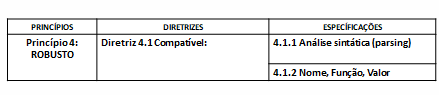
\includegraphics[scale=0.9]{Robusto.png}}
\end{center}

Mas na frente na seção 5, serão detalhadas as especificações, porém, com o que já foi apresentado, é visto que as diretrizes são bem extensa e abrange quase todas as formas de acessibilidade existentes. Agora é preciso só que os programadores se propõem a seguir os quatro princípios básicos ditos anteriormente, com a meta de fazer tal atividade em seus trechos de códigos, fazendo com que todas as pessoas consigam manipular os seus sites, sem haver nenhum tipo de discriminação por partes dos programadores e dos produtores de conteúdos.

\subsection{Avaliação de Acessibilidade de Sites}
Nesta subseção são apresentados artigos sobre avaliação de acessibilidade de sites de diferentes campos.  Vamos começar pelo artigo [1], onde seus autores avaliaram 107 sites educacionais no Brasil. Eles verificaram a existência de um grande descaso relacionado com a inclusão digital, pois apenas 14,02\% possuem atalhos no teclado, 22,43\% possuem a opção de alto contraste, 41,12\% possuem a barra de acessibilidade, 36,45\% possuem o mapa de sitio e só 14,02\% possuem páginas com descrições com os recursos de acessibilidade. Isso nos mostra que, segundo os pesquisadores, os resultados obtidos apontam para um elevado descaso com a inclusão digital em relação às pessoas com deficiência, de forma que o nível de adoção dos padrões de acessibilidade é extremamente baixo nos portais das Instituições Federais de Ensino, algo que é bastante ruim, pois nem mesmo os próprios sites governamentais possuem a acessibilidade, ainda que existam leis que exigem a acessibilidade nos sites.

Já em [7], foi feito uma analise da acessibilidade dos sites governamentais da Arábia Saudita pela segunda vez em seis anos, seguiram alguns pontos da WCAG para a sua investigação das ditas plataformas digitais. Dentre os pontos que foram analisados estão uma boa informação de conteúdo não textual e seus relacionamentos, a existência de contraste, imagens de texto, usando o vídeo de libras, atalhos de teclado, interrupções e uma boa sequência significativa. Segundo eles, os resultados da avaliação são promissores e indicam um aumento da conscientização para acessibilidade da web. Isso pode ter acontecido pelo aumento da consciência de desenvolver serviços de governo eletrônico acessíveis, impostos pelo governo, o que implica a existência de padrões que promovem acessibilidade web na Arábia Saudita. No entanto, os autores sugerem alguns pontos para melhorar a acessibilidade do governo governamental saudita sites, incluindo aumentar apoio do governo, fornecendo o treinamento necessário para atender aos requisitos de acessibilidade dos sites.

Já o artigo [9] tinha como objetivo investiga o quão bem os sites de governo eletrônico móvel saudita cumprem os padrões de usabilidade e diretrizes de acessibilidade recomendados das diretrizes de acessibilidades dos conteúdos da Web (WCAG). Chegaram a conclusão que há problemas de usabilidade e acessibilidade que afetam o desempenho de sites governamentais. Dentre os pontos existentes na diretriz, foram analisados a existência de texto alternativo as imagens, alto contraste no texto, descrição dos link, formulários de fácil compreensão e textos, em gerais, que favoreçam o uso dos leitores de tela, que são usados caso tenham uma boa sequência significativa.

O artigo [11] tinha como objetivo deste avaliar a acessibilidade dos vídeos publicados no YouTube pelas melhores universidades do mundo com base no cumprimento das WCAG. No caso a pesquisa foi feita em cima 91421 vídeos de 113 universidades do mundo. Os resultados deste estudo mostram que embora apenas 17\% do total de vídeos publicados tenham legendas associadas, mas o cumprimento deste critério de sucesso tem melhorado ao longo dos anos. Porém, se for visto em relação à linguagem de sinais, à descrição de áudio ou à descrição de áudio estendida com vídeos, a acessibilidade é zero, pois todos os vídeos dos sites são puxados da plataforma YouTube, que não possuem essas funcionalidades.

A seguir, na tabela 1, vemos a comparação dos artigos citados nessa seção com as características da diretriz WCAG.\\

Tabela 1 - Análise características das diretrizes com os artigos.
\begin{center}
	\begin{tabular}{cc}
		\hline
		Artigos & Diretrizes cumpridas\\
		\hline
		Artigo [1] & 1.2.3/1.2.5/1.2.7/1.4.3/1.4.5/1.4.6/1.4.9/2.1.1/2.1.2/2.1.3\\
		Artigo [7] & 1.2.6/1.3.2/1.4.3/1.4.5/1.4.6/1.4.9/2.1.1/2.1.2/2.1.3/2.2.4\\
		Artigo [9] & 1.2.8/1.2.9/1.3.2/1.4.3/1.4.5/1.4.6/1.4.9/4.1.2\\
		Artigo [11] & 1.1.1/1.2.1/1.2.2/1.2.3/1.2.4/1.2.5/1.2.6\\
		\hline
	\end{tabular}
\end{center}

Já o artigo [8] definiu o termo acessibilidade, dizendo que quando aplicado à web, diz respeito ao desenvolvimento de um design útil para facilitar o acesso a um número mais significativo de usuários. Uma página web acessível permitirá que os usuários com alguma deficiência permanente ou temporária recebam e entendam o conteúdo de um site, bem como possam navegar em tudo corretamente. Nesse artigo foi analisado um método heurístico existente para investigar o nível de acessibilidade de 40 sites, incluindo os de 30 universidades da América Latina e 10 sites entre os mais visitados, segundo o ranking Alexa. Foram analisados em relação aos usuários com baixa visão, o método utilizado foi proposto por Brajnik e WCAG 2.1, aplicando uma avaliação manual e se enquadra no grupo ''Testes de Triagem de Barreiras''. Esta técnica consiste em priorizar os impactos das barreiras de acordo com o contexto aplicado. O método permite a identificação da gravidade de cada barreira; este método heurístico busca identificar problemas de acessibilidade. A finalidade do artigo era analisar as barreiras existentes nas plataformas, com o objetivo de ajudar os programadores a ajeitarem esses impeditivos nessas plataformas, além de influenciar sites que ainda serão criados no futuro. Assim, o artigo concluiu que muitas dessas páginas web analisadas, violaram os princípios da diretriz WCAG, totalizando 241 barreiras que impossibilitam o manuseio simples e fácil do site.

\section{TIPOS DE DEFICIÊNCIA}
\section{ANÁLISE DA DIRETRIZ WCAG}
\section{ANÁLISE DOS SITES DE NOTÍCIA}
\section{CONCLUSÃO}
\section*{REFERÊNCIAS}
\addcontentsline{toc}{section}{Referência}
\hspace{-0.05\textwidth}
\begin{minipage}{1\textwidth}
[1] M. Campoverde-Molina, S. Lujan-Mora, e L. Valverde Gracia, "Empirical Studies on Web Accessibility of Educational Websites: A Systematic Literature Review" em IEEEAcess, Abril de 2020.
\end{minipage}\\[0.5cm]
[2] D. Luís Arenhardt, T. Stefanel Franchi, e S. Medianeira Flores Costa, M. Zampieri Grohmann, "Acessibilidade digital: Uma análise em portais de Instituições Federais de Educação do Brasil" em Education Policy Analysis Archives, Abril de 2017.\\[0.5cm] [3] P. Acosta-Vargas, T. Acosta, e S. Luján-Mora, "Challenges to Assess Accessibility in Higher A Comparative Study of Latin America Universities" em IEEEAcess, Março de 2018.\\[0.5cm] [4] E. M. Molanes-López, A. Rodriguez-Ascaso, E. Letón, E J. Pérez-Martín, "Assessment of Video Accessibility by Students of a MOOC on Digital Materials for All a MOOC on Digital Materials for All" em IEEEAcess, Maio de 2021.\\[0.5cm] [5] A. Ismail, K. S. Kuppusamy, "Web accessibility investigation and identification of major issues of higher education websites with statistical measures - A case study of college websites" em Journal of King Saud University – Computer and Information Sciences, Março de 2019.\\[0.5cm] [6] A. Ismail, K. S. Kuppusamy, "Accessibility of Indian universities homepages An exploratory study" em Journal of King Saud University – Computer and Information Sciences, Junho de 2016.\\[0.5cm] [7] H. S. Al-Khalifa, I. Baazeem e R. Alamer1, "Revisiting the accessibility of Saudi Arabia government websites" em Universal Access in the Information Society, Setembro de 2016.\\[0.5cm] [8] P. Acosta-Vargas, T. Acosta, e S. Luján-Mora, "A Heuristic Method to Evaluate Web Accessibility for Users With Low Vision" em IEEEAcess, Março de 2018.\\[0.5cm] [9] H. O. Al-Sakran, M. A, Alsudairi "Usability and Accessibility Assessment of Saudi Arabia Mobile E-Government Websites" em IEEEAcess, Março de 2021.\\[0.5cm] [10] B. Caldwell, M. Cooper, L. Guarino Reid, G. Vanderheiden, W. Chisholm, J. Slatin e J. White, Consórcio W3C(2008), "Diretrizes de Acessibilidade para Conteúdo Web (WCAG)2.0", Acesso em: 11 jun. 2021. [Online]. Disponível: https://www.w3.org/Translations/WCAG20-pt-PT/WCAG20-pt-PT-20141024/\\[0.5cm] [11] T. Acosta, P. Acosta Vargas, J. Zambrano Miranda e S. Luján Mora, "Web Accessibility Evaluation of Videos Published on YouTube by Worldwide Top-Ranking Universities" em IEEEAcess, Junho de 2020.

\end{titlepage}
\end{document}